\begin{figure}[!ht]
    \centering
    \begin{subfigure}[t]{0.3\textwidth}
        \centering
        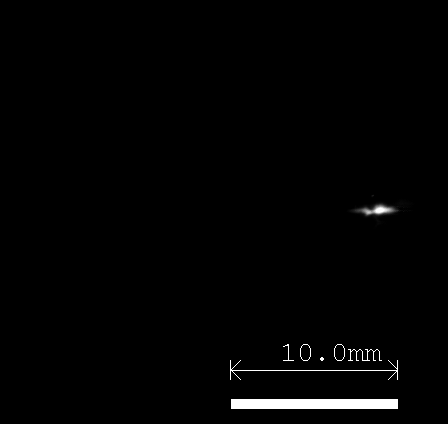
\includegraphics[width=\textwidth]{assets/4 experiments/V1 Spark Ignition Frames/LSP142_SPRK15_Fr32.png}
        \caption{\qty{3.2}{ms}}
        %\label{fig:V1_ignition_frames_16}
    \end{subfigure}
    \hfill
    \begin{subfigure}[t]{0.3\textwidth}
        \centering
        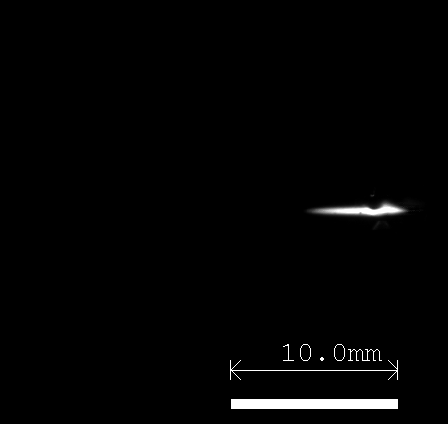
\includegraphics[width=\textwidth]{assets/4 experiments/V1 Spark Ignition Frames/LSP142_SPRK15_Fr33.png}
        \caption{\qty{3.3}{ms}}
        %\label{fig:ignition_frames_17}
    \end{subfigure}
    \hfill
    \begin{subfigure}[t]{0.3\textwidth}
        \centering
        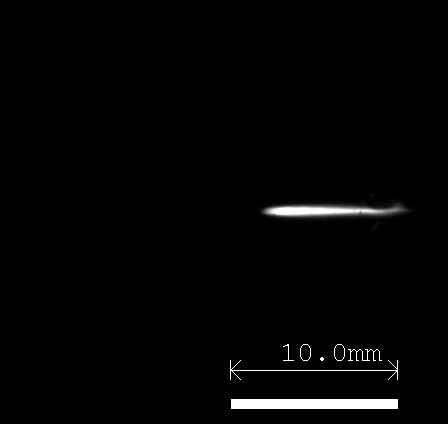
\includegraphics[width=\textwidth]{assets/4 experiments/V1 Spark Ignition Frames/LSP142_SPRK15_Fr35.png}
        \caption{\qty{3.5}{ms}}
        %\label{fig:ignition_frames_18}
    \end{subfigure}
    \begin{subfigure}[t]{0.3\textwidth}
        \centering
        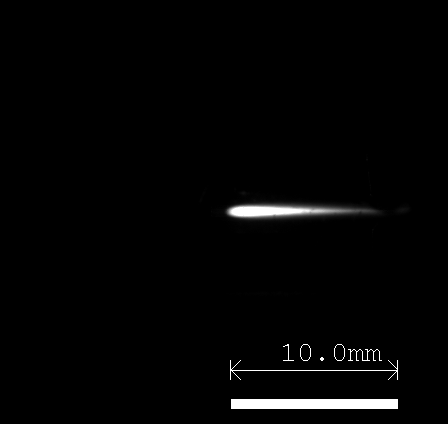
\includegraphics[width=\textwidth]{assets/4 experiments/V1 Spark Ignition Frames/LSP142_SPRK15_Fr38.png}
        \caption{\qty{3.8}{ms}}
        %\label{fig:ignition_frames_19}
    \end{subfigure}
    \hfill
    \begin{subfigure}[t]{0.3\textwidth}
        \centering
        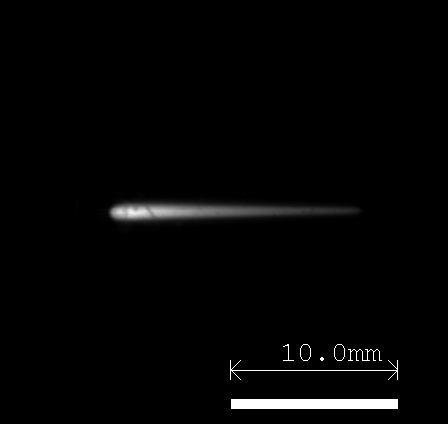
\includegraphics[width=\textwidth]{assets/4 experiments/V1 Spark Ignition Frames/LSP142_SPRK15_Fr69.png}
        \caption{\qty{6.9}{ms}}
        %\label{fig:ignition_frames_20}
    \end{subfigure}
    \caption{TO CHANGE: CW LSP spark initiation with V2: \qty{350}{W}, \qty{20}{bar}. \shotsettings{LSP385\_V2\_CW1}}
    \label{fig:V1_spark_initiation_frames}
\end{figure}